\subsection*{Проект <<Доставка товаров на примере маркетплейса Ozon>>}
\addcontentsline{toc}{subsection}{Проект <<Доставка товаров на примере маркетплейса Ozon>>}

\textbf{Задание:}\\
Имеется база данных адресов клиентов и адресов пунктов выдачи Санкт-Петербурга (количество адресов детерминировано).\\ 

Клиент может забрать заказ из пункта выдачи, либо заказать доставку непосредственно себе домой (адреса клиентов генерируются динамически).\\

Заказ оформляется с заданной интенсивностью.\\

Товар находится на складе, оттуда его везут либо в пункт выдачи, либо отправляют доставкой клиенту.\\

Машина с товарами отправляется со склада тогда, когда достигнут минимальный размер или объем партии отправляемых заказов или если наступило критическое время отправки заказа (неделя до даты доставки в пункт выдачи), для реализации этой механики каждому заказу присваивается размер (значение от 1 до 100 в зависимости от объема и веса товара) и примерная дата доставки в пункт выдачи.\\

Имеется возможность оформления возврата и вывоза возвращенных и забытых на пункте выдачи товаров на склад (предполагается, что товары не имеют брака).\\

Имеется склад, который реализует починку товаров.\\

\textbf{Решение:}\\
Для начала создаем модель, единицами измерения времени модели указываем часы.\\

На следующем шаге необходимо создать популяцию агентов.\\

Первая популяция – популяция обычных складов, данные которой загружаются из базы данных (файла excel, в котором указаны координаты складов, их названия и число грузовиков, имеющихся в распоряжении). (Рисунок \ref{fig:ozon1}, \ref{fig:ozon2})

\newpage

\begin{figure}[h]
	\centering 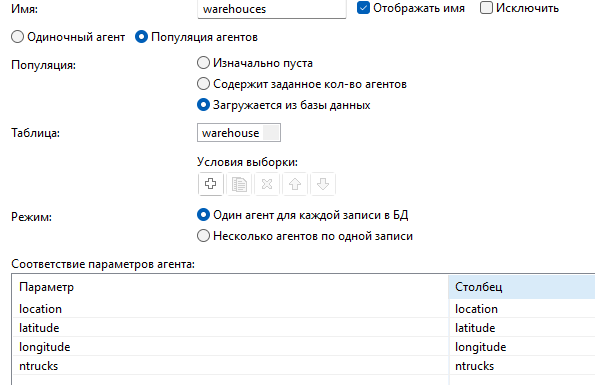
\includegraphics[scale=0.5]{ozon1}
	\caption{Склады}
	\label{fig:ozon1}
\end{figure}

\begin{figure}[h]
	\centering 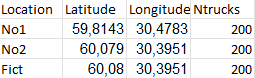
\includegraphics[scale=1]{ozon2}
	\caption{Данные}
	\label{fig:ozon2}
\end{figure}

Вторая популяция – это популяция грузовиков, которые хранятся на складах. (Рисунок \ref{fig:ozon3})
\begin{figure}[h]
	\centering 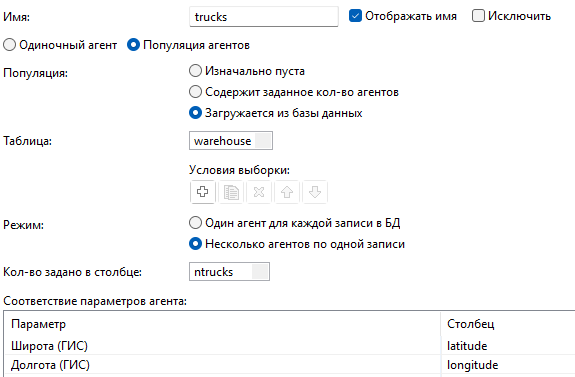
\includegraphics[scale=0.6]{ozon3}
	\caption{Грузовики}
	\label{fig:ozon3}
\end{figure}

\newpage

Третья популяция – популяция пунктов выдачи, данные которой загружаются из базы данных (файла excel, в котором указаны координаты пунктов выдачи и их названия). (Рисунок \ref{fig:ozon4}, \ref{fig:ozon5})
\begin{figure}[h]
	\centering 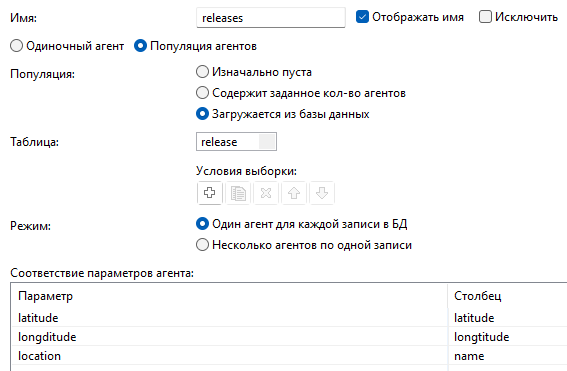
\includegraphics[scale=0.6]{ozon4}
	\caption{Пункты выдачи}
	\label{fig:ozon4}
\end{figure}

\begin{figure}[h]
	\centering 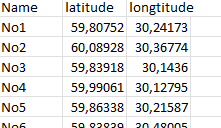
\includegraphics[scale=1]{ozon5}
	\caption{Данные}
	\label{fig:ozon5}
\end{figure}

Четвертая популяция –  популяция складов, на которых осуществляется починка, в нашем случае она состоит из одного элемента, у которого указаны координаты и название, данный склад не имеет грузовики в своем распоряжении. (Рисунок \ref{fig:ozon6})
\begin{figure}[h]
	\centering 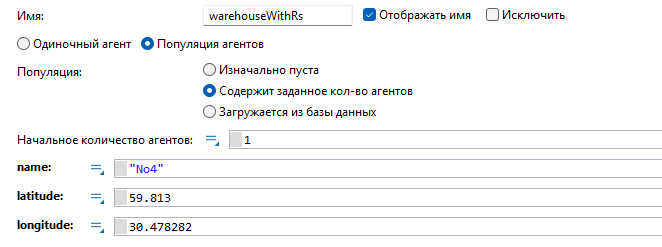
\includegraphics[scale=0.6]{ozon6}
	\caption{Склад с починкой}
	\label{fig:ozon6}
\end{figure}

\newpage

Пятая популяция – популяция адресов клиентов, данная популяция изначально пуста, ее элементы генерируются при помощи события. (Рисунок \ref{fig:ozon7})
\begin{figure}[h]
	\centering 
\includegraphics[scale=0.6]{ozon7}
	\caption{Доставки}
	\label{fig:ozon7}
\end{figure}

Шестая популяция – доставки, данная популяция также является изначально пустой, ее элементы также генерируются при помощи события. (Рисунок \ref{fig:ozon8})
\begin{figure}[h]
	\centering 
\includegraphics[scale=0.6]{ozon8}
	\caption{Дома}
	\label{fig:ozon8}
\end{figure}

\begin{figure}[h]
	\centering 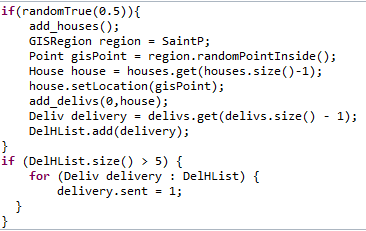
\includegraphics[scale=0.8]{ozon9}
	\caption{Событие, генерирующее элементы популяций}
	\label{fig:ozon9}
\end{figure}

\newpage

Движение грузовиков по карте осуществляется при помощи диаграммы состояний. (Рисунок \ref{fig:ozon10})
\begin{figure}[h]
	\centering 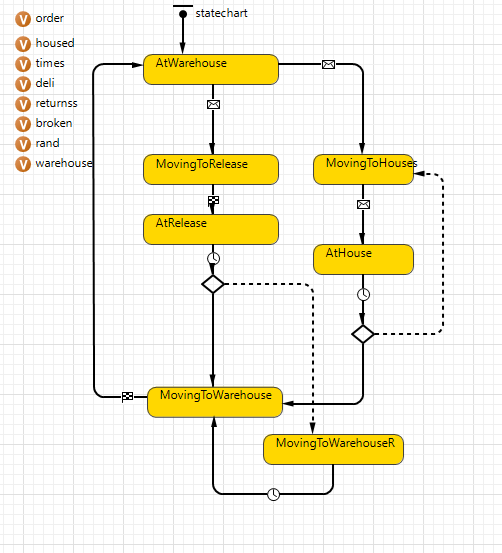
\includegraphics[scale=0.6]{ozon10}
	\caption{Диаграмма состояний грузовиков}
	\label{fig:ozon10}
\end{figure}

В данной диаграмме происходит следующее: при получении сообщения типа заказ грузовик выезжает на пункт выдачи, который его вызвал, в нем он разгружает товар и забирает возвращенный и сломанный товар, после чего, если сломанного товара на складе не было, то грузовик уезжает на ближайший склад, а если был, то отвозит его на склад с починкой, после чего уезжает на склад, в котором находится меньше всего грузовиков; при получении сообщения типа доставка, грузовик едет к ближайшему дому, на адрес которого была заказана доставка, после чего объезжает еще 4 дома, которые отправили сообщение типа доставка, а затем уезжает на ближайший склад.\\

Условия отправки сообщений типа заказ реализуются в событии, расположенном в агенте популяции пунктов выдачи. В нем осуществляется условие того, что машина с товарами отправляется со склада тогда, когда достигнут минимальный размер или объем партии отправляемых заказов или если наступило критическое время отправки заказа. (Рисунок \ref{fig:ozon11})

\newpage

\begin{figure}[h]
	\centering 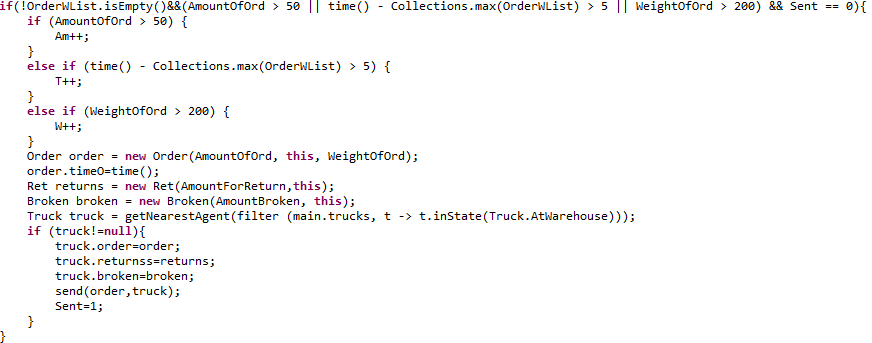
\includegraphics[scale=0.6]{ozon11}
	\caption{Отправка сообщений о заказе}
	\label{fig:ozon11}
\end{figure}

Данное событие задействует еще одно событие – увеличение количества заказов, веса, количества возвратов, сломанных вещей, установление срока отправки заказа. (Рисунок \ref{fig:ozon12})

\begin{figure}[h]
	\centering 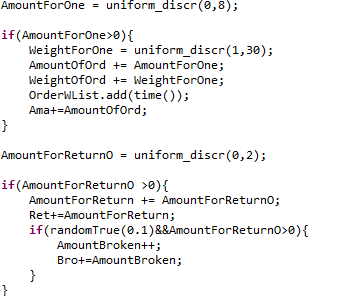
\includegraphics[scale=0.6]{ozon12}
	\caption{Изменение параметров}
	\label{fig:ozon12}
\end{figure}

Условия отправки сообщений типа доставка осуществляется в событии, расположенном в агенте популяции доставка. (Рисунок \ref{fig:ozon13})

\begin{figure}[h]
	\centering 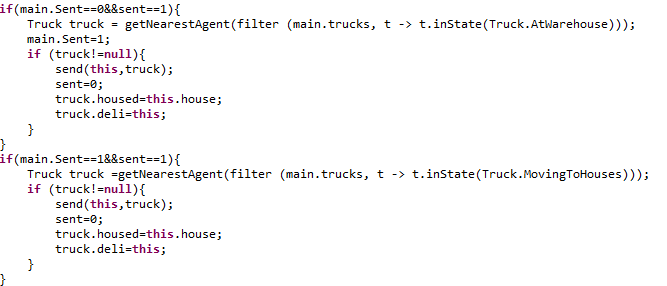
\includegraphics[scale=0.435]{ozon13}
	\caption{Отправка сообщений о доставке}
	\label{fig:ozon13}
\end{figure}

\newpage

При запуске модель будет выглядеть следующим образом. (Рисунок \ref{fig:ozon14})

\begin{figure}[h]
	\centering 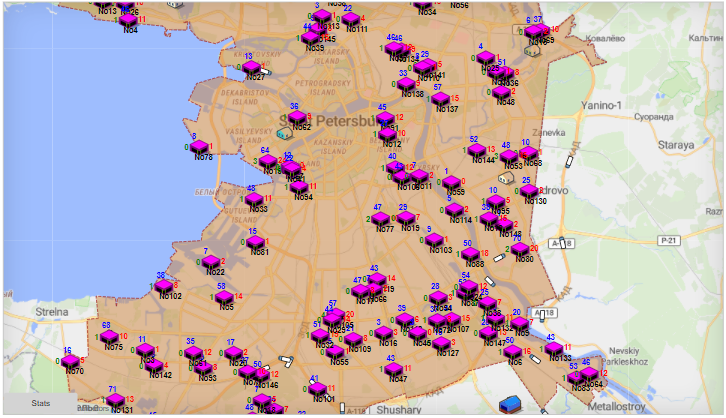
\includegraphics[scale=0.6]{ozon14}
	\caption{Работа модели}
	\label{fig:ozon14}
\end{figure}

Теперь необходимо собрать статистику и сделать выводы относительно проделанной работы.\\

При изначальных параметрах статистика по времени ожидания доставки, времени ожидания заказа, количеству машин на складах, количеству доставок и заказов, количеству сломанных, возвращенных и полученных заказов, отправок заявок на получение заказа по предельно допустимому количеству, весу и сроку доставки выглядит следующим образом. (Рисунок \ref{fig:ozon15})

\begin{figure}[h]
	\centering 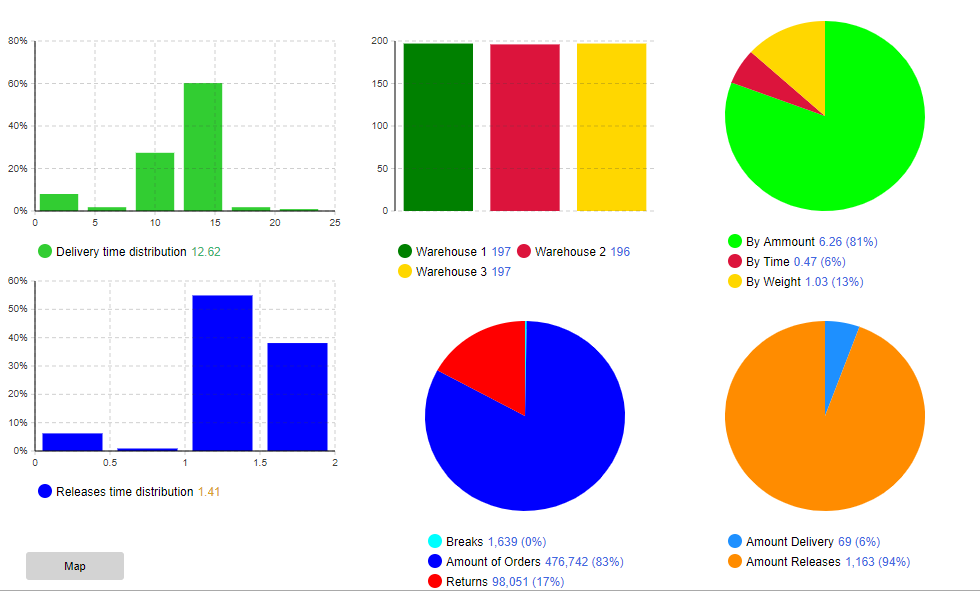
\includegraphics[scale=0.45]{ozon15}
	\caption{Начальная статистика}
	\label{fig:ozon15}
\end{figure}

\newpage

Если мы уменьшим количество заказов, поступающих за час, то  теперь основным критерием, по которому будут отправляться заявки на заказ, станет вес, время ожидания пунктов выдачи уменьшится, время ожидания  доставок практически не изменится. (Рисунок \ref{fig:ozon16})

\begin{figure}[h]
	\centering 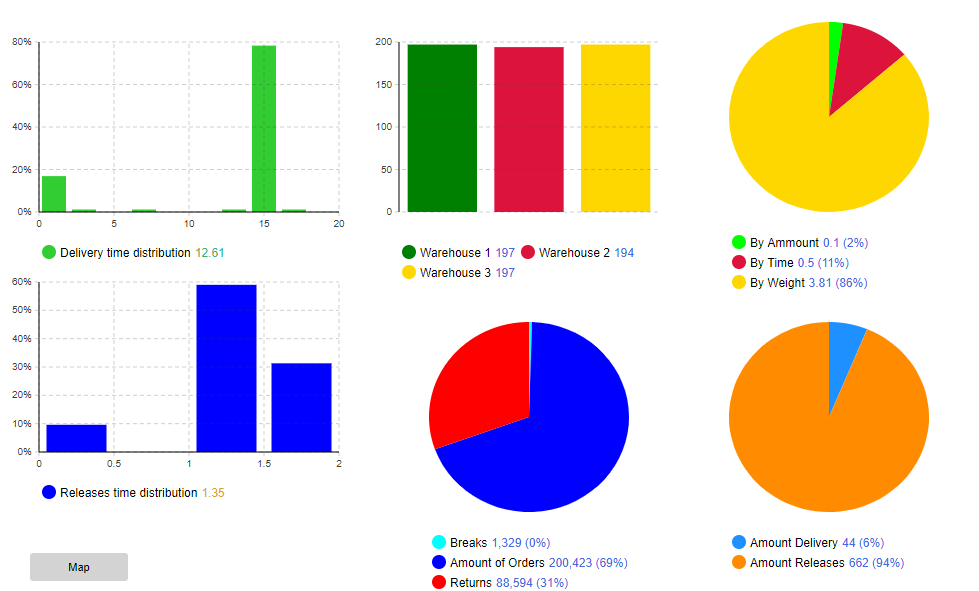
\includegraphics[scale=0.45]{ozon16}
	\caption{Уменьшение интенсивности заказов}
	\label{fig:ozon16}
\end{figure}

Если мы увеличим интенсивность создания заказов, то основным критерием, по которому будут отправляться заявки на заказ, станет количество, время ожидания пунктов выдачи увеличится, время ожидания  доставок тоже увеличится. (Рисунок \ref{fig:ozon17})

\begin{figure}[h]
	\centering 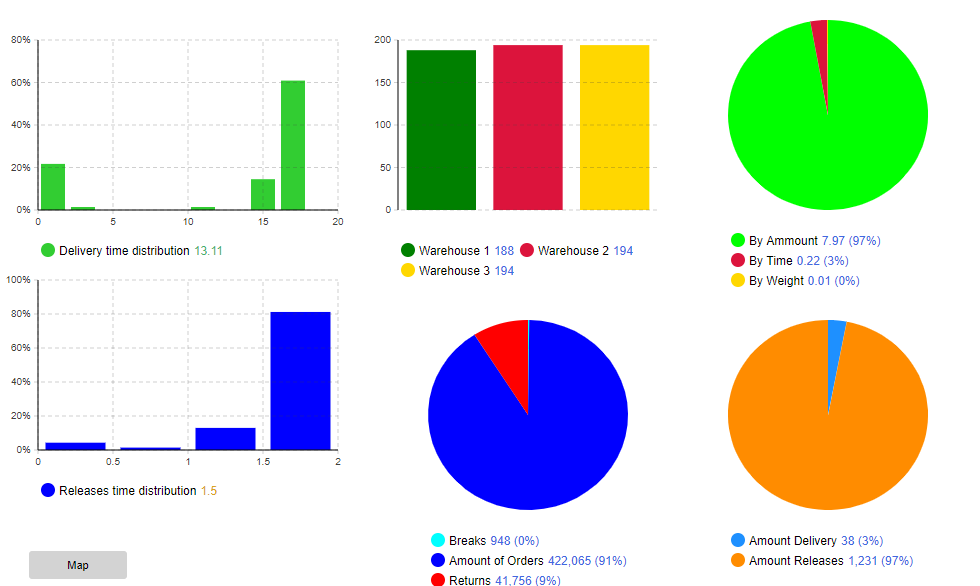
\includegraphics[scale=0.45]{ozon17}
	\caption{Увеличение интенсивности заказов}
	\label{fig:ozon17}
\end{figure}

При увеличении вероятности заказа доставки увеличится время ожидания доставки и время ожидания заказа. (Рисунок \ref{fig:ozon18})

\newpage

\begin{figure}[h]
	\centering 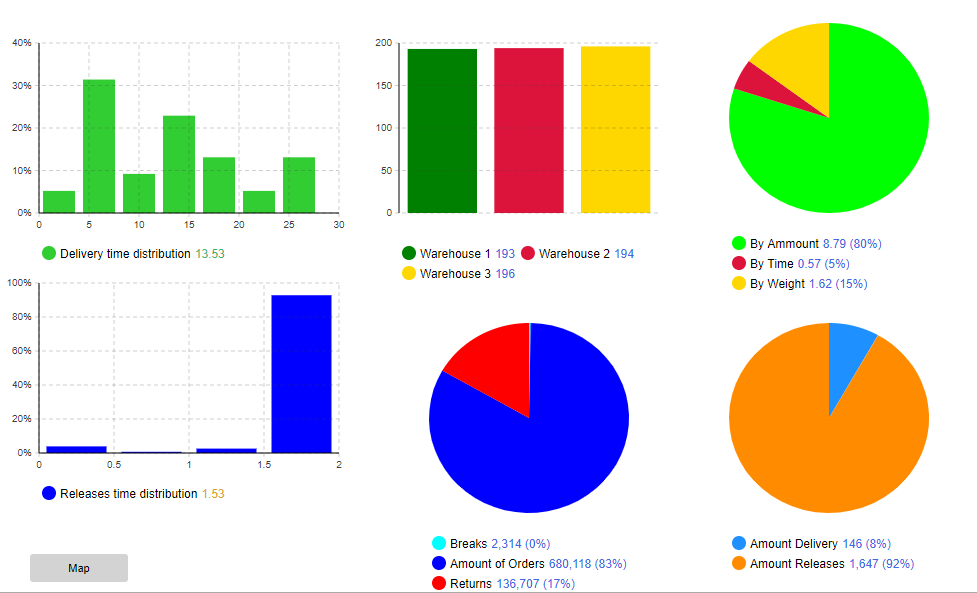
\includegraphics[scale=0.45]{ozon18}
	\caption{Увеличение вероятности оформления доставки}
	\label{fig:ozon18}
\end{figure}

При уменьшении вероятности оформления доставки уменьшится время ожидания доставки, время ожидания заказа практически не изменится. (Рисунок \ref{fig:ozon19})

\begin{figure}[h]
	\centering 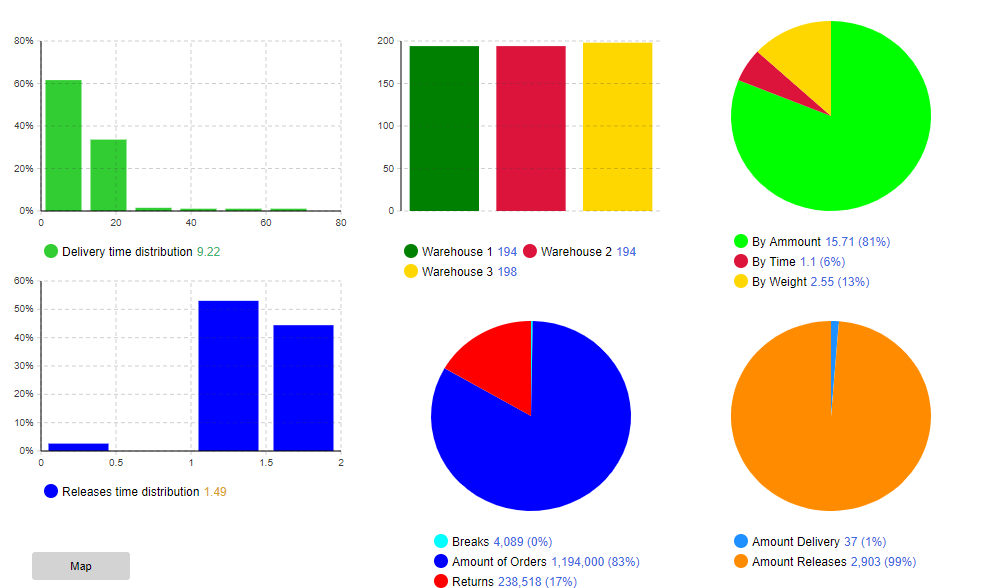
\includegraphics[scale=0.45]{ozon19}
	\caption{Уменьшение вероятности оформления доставки}
	\label{fig:ozon19}
\end{figure}

Добавим еще одну круговую диаграмму, которая будет показывать, какое количество грузовиков задействовано в настоящий момент. При начальных параметрах (на каждом складе находится 200 машин) диаграмма показывает, что используются лишь 5-8\% от всего числа машин. (Рисунок \ref{fig:ozon20})

\newpage

\begin{figure}[h]
	\centering 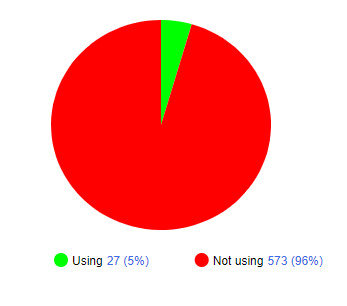
\includegraphics[scale=0.6]{ozon20}
	\caption{Нагрузка на грузовики}
	\label{fig:ozon20}
\end{figure}

Этот результат говорит о том, что большая часть машин не используется. Чтобы приблизить ситуацию к реальности, необходимо изменить количество машин на складах. При количестве грузовиков на каждом складе равном 20 используется 0т 30 до 65\% транспорта, что говорит о том, что не используемых грузовиков практически нет и такое количество является оптимальным. (Рисунок \ref{fig:ozon21})

\begin{figure}[h]
	\centering 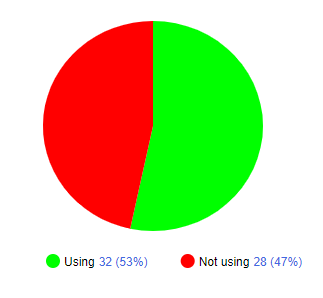
\includegraphics[scale=0.6]{ozon21}
	\caption{Нагрузка на грузовики при уменьшении их количества}
	\label{fig:ozon21}
\end{figure}

Также можно посмотреть влияние других параметров на статистику, однако характер этих изменений будет похож на рассмотренный ранее.\\

Таким образом, нами была реализована модель доставки товаров на примере маркетплейса Ozon, была собрана необходимая для анализа статистика, был проведен анализ поведения модели при изменении параметров.\\